%--------------------------------------------------------------------%
%
% Berkas utama templat LaTeX.
%
% author Petra Barus, Peb Ruswono Aryan
%
%--------------------------------------------------------------------%
%
% Berkas ini berisi struktur utama dokumen LaTeX yang akan dibuat.
%
%--------------------------------------------------------------------%

\documentclass[12pt, a4paper, onecolumn, oneside, final]{report}

%-------------------------------------------------------------------%
%
% Konfigurasi dokumen LaTeX untuk laporan tesis IF ITB
%
% @author Petra Novandi
%
%-------------------------------------------------------------------%
%
% Berkas asli berasal dari Steven Lolong
%
%-------------------------------------------------------------------%

% Ukuran kertas
\special{papersize=210mm,297mm}

% Setting margin
\usepackage[top=3cm,bottom=2.5cm,left=4cm,right=2.5cm]{geometry}

\usepackage{mathptmx}

% Judul bahasa Indonesia
\usepackage[bahasa]{babel}

% Format citation
\usepackage[backend=bibtex,citestyle=authoryear]{biblatex}

\usepackage[utf8]{inputenc}
\usepackage{graphicx}
\usepackage{titling}
\usepackage{blindtext}
\usepackage{sectsty}
\usepackage{chngcntr}
\usepackage{etoolbox}
\usepackage{hyperref}       % Package untuk link di daftar isi.
\usepackage{titlesec}       % Package Format judul
\usepackage{parskip}

% Line satu setengah spasi
\renewcommand{\baselinestretch}{1.5}

% Setting judul
\chapterfont{\centering \Large}
\titleformat{\chapter}[display]
  {\Large\centering\bfseries}
  {\chaptertitlename\ \thechapter}{0pt}
    {\Large\bfseries\uppercase}

% Setting nomor pada subbsubsubbab
\setcounter{secnumdepth}{3}

\makeatletter

\makeatother

% Counter untuk figure dan table.
\counterwithin{figure}{section}
\counterwithin{table}{section}

%--------------------------------------------------------------------%
%
% Hypenation untuk Bahasa Indonesia
%
% @author Petra Barus
%
%--------------------------------------------------------------------%
%
% Secara otomatis LaTeX dapat langsung memenggal kata dalam dokumen,
% tapi sering kali terdapat kesalahan dalam pemenggalan kata. Untuk
% memperbaiki kesalahan pemenggalan kata tertentu, cara pemenggalan
% kata tersebut dapat ditambahkan pada dokumen ini. Pemenggalan
% dilakukan dengan menambahkan karakter '-' pada suku kata yang
% perlu dipisahkan.
%
% Contoh pemenggalan kata 'analisa' dilakukan dengan 'a-na-li-sa'
%
%--------------------------------------------------------------------%

\hypenation {
	% A
	%
	a-na-li-sa
	a-pli-ka-si

	% B
	%
	be-be-ra-pa
	ber-ge-rak

	% C
	%
	ca-ri

	% D
	%
	da-e-rah
	di-nya-ta-kan
	de-fi-ni-si

	% E
	%
	e-ner-gi
	eks-klu-sif

	% F
	%
	fa-si-li-tas

	% G
	%
	ga-bung-an

	% H
	%
	ha-lang-an

	% I
	% 
	i-nduk

	% J
	%
	ka-me-ra
	kua-li-tas

	% K
	%

	% L
	%

	% M
	%

	% N
	%

	% O
	%

	% P
	%

	% Q
	%

	% R
	%

	% S
	%

	% T
	% 

	% U
	%

	% V
	%

	% W
	%

	% X
	%

	% Y
	% 

	% Z
	%
}


\makeatletter
\makeatother

\bibliography{references}

\begin{document}
\sloppy

    %Basic configuration
    \title{Penggunaan Model Transformer Pada \textit{Audiovisual Speech Recognition} Untuk Bahasa Indonesia}
    \date{}
    \author{
        Gugy Lucky Khamdani \\
        NIM: 23517041
    }

    \pagenumbering{roman}
    \setcounter{page}{0}

    \clearpage
\pagestyle{empty}

\begin{center}
\smallskip

    \Large \bfseries \MakeUppercase{\thetitle}
    \vfill

    \Large Laporan Tugas Akhir
    \vfill

    \large Disusun sebagai syarat kelulusan tingkat sarjana
    \vfill

    \large Oleh

    \Large \theauthor

    \vfill
    \begin{figure}[h]
        \centering
      	
\includegraphics[width=0.15\textwidth]{resources/cover-ganesha.jpg}
    \end{figure}
    \vfill

    \large
    \uppercase{
        Program Studi Teknik Informatika \\
        Sekolah Teknik Elektro dan Informatika \\
        Institut Teknologi Bandung
    }

    November 2016

\end{center}

\clearpage


    \pagestyle{plain}

	\titlespacing{\chapter}{0pt}{-20pt}{15pt}
	
    \titleformat{\chapter}[hang]
    	{\bfseries \centering \Large \MakeUppercase}
    	{}
    	{1em}
    	{}

    % \clearpage
\chapter*{ABSTRAK}
\addcontentsline{toc}{chapter}{Abstrak}

%taruh abstrak bahasa indonesia di sini
\blindtext
\clearpage
    % \clearpage
\chapter*{\textit{ABSTRACT}}
\addcontentsline{toc}{chapter}{Abstract}

\begin{center}
	\begin{spacing}{1}
    \Large \bfseries \textit{\MakeUppercase{Transformer Model For Audiovisual Speech Recognition in Bahasa Indonesia}}
    \end{spacing}
    
    \Large \textit{By} \\
    \begin{spacing}{1}
		\bfseries \Large \theauthor \\
		\textit{(Master's Program in Informatics/Computer Science)}
    \end{spacing}
\end{center}

%taruh abstrak bahasa inggris di sini
\begin{spacing}{1}
	{\itshape
		\blindtext

		\blindtext
		
		\textbf{Keywords}: keyword1, keyword2, keyword3, keyword4
	}
\end{spacing}
\clearpage
    \clearpage
\pagestyle{empty}

\begin{center}
\smallskip

	\begin{spacing}{1}
    	\Large \bfseries \MakeUppercase{Judul Tesis: \thetitle}
    \end{spacing}
    \vfill

    \large Oleh \\
    \begin{spacing}{1}
		\bfseries \Large \theauthor \\
		(Program Studi Magister Informatika)  
    \end{spacing}

    \large Institut Teknologi Bandung \\

    \vfill
    \normalsize \normalfont
    Menyetujui \\
    Pembimbing
    
    tanggal 20 Juli 2016.

    \vfill
    %\setlength{\tabcolsep}{12pt}
    %\begin{tabular}{c@{\hskip 0.5in}c}
    %    Pembimbing I, & Pembimbing II \\
    %    & \\
    %    & \\
    %    & \\
    %    & \\
    %    Nama dan Gelar Pembimbing I & Nama dan Gelar Pembimbing II \\
    %    NIP 123456789 & NIP 123456789 \\
    %\end{tabular}
    
    Nama dan Gelar Pembimbing I \\
    NIP 123456789

\end{center}
\clearpage

    % \chapter*{Pedoman Penggunaan Tesis}
\addcontentsline{toc}{chapter}{Pedoman Penggunaan Tesis}

Gunakan bagian ini untuk memberikan ucapan terima kasih kepada semua pihak yang secara langsung atau tidak langsung membantu penyelesaian tugas akhir, termasuk pemberi beasiswa jika ada. Utamakan untuk memberikan ucapan terima kasih kepada tim pembimbing tugas akhir dan staf pengajar atau pihak program studi, bahkan sebelum mengucapkan terima kasih kepada keluarga. Ucapan terima kasih sebaiknya bukan hanya menyebutkan nama orang saja, tetapi juga memberikan penjelasan bagaimana bentuk bantuan/dukungan yang diberikan. Gunakan bahasa yang baik dan sopan serta memberikan kesan yang enak untuk dibaca. Sebagai contoh: “Tidak lupa saya ucapkan terima kasih kepada teman dekat saya, Tito, yang sejak satu tahun terakhir ini selalu memberikan semangat dan mengingatkan saya apabila lengah dalam mengerjakan Tugas Akhir ini. Tito juga banyak membantu mengoreksi format dan layout tulisan. Apresiasi saya sampaikan kepada pemberi beasiswa, Yayasan Beasiswa, yang telah memberikan bantuan dana kuliah dan biaya hidup selama dua tahun. Bantuan dana tersebut sangat membantu saya untuk dapat lebih fokus dalam menyelesaikan pendidikan saya. ....”. Ucapan permintaan maaf karena kekurangsempurnaan hasil Tugas Akhir tidak perlu ditulis.

    % \chapter*{Kata Pengantar}
\addcontentsline{toc}{chapter}{Kata Pengantar}

Gunakan bagian ini untuk memberikan ucapan terima kasih kepada semua pihak yang secara langsung atau tidak langsung membantu penyelesaian tugas akhir, termasuk pemberi beasiswa jika ada. Utamakan untuk memberikan ucapan terima kasih kepada tim pembimbing tugas akhir dan staf pengajar atau pihak program studi, bahkan sebelum mengucapkan terima kasih kepada keluarga. Ucapan terima kasih sebaiknya bukan hanya menyebutkan nama orang saja, tetapi juga memberikan penjelasan bagaimana bentuk bantuan/dukungan yang diberikan. Gunakan bahasa yang baik dan sopan serta memberikan kesan yang enak untuk dibaca. Sebagai contoh: “Tidak lupa saya ucapkan terima kasih kepada teman dekat saya, Tito, yang sejak satu tahun terakhir ini selalu memberikan semangat dan mengingatkan saya apabila lengah dalam mengerjakan Tugas Akhir ini. Tito juga banyak membantu mengoreksi format dan layout tulisan. Apresiasi saya sampaikan kepada pemberi beasiswa, Yayasan Beasiswa, yang telah memberikan bantuan dana kuliah dan biaya hidup selama dua tahun. Bantuan dana tersebut sangat membantu saya untuk dapat lebih fokus dalam menyelesaikan pendidikan saya. ....”. Ucapan permintaan maaf karena kekurangsempurnaan hasil Tugas Akhir tidak perlu ditulis.

    
    \titleformat*{\section}{\centering\bfseries\Large\MakeUpperCase}
    
    \renewcommand{\cftchapfont}{\normalfont}
    \renewcommand{\cftchappagefont}{\normalfont}
    \clearpage
    \addcontentsline{toc}{chapter}{Daftar Isi}
    \renewcommand*{\contentsname}{DAFTAR ISI}
    \renewcommand{\cftchapdotsep}{\cftdotsep}
    \renewcommand{\cftdot}{.}
    \titleformat{\section}{\bfseries\sffamily\large}{\thesection.}{\hspace{1cm}}{}%
 	\titleformat{\subsection}{\bfseries\sffamily\large}{\thesection.}{\hspace{1cm}}{}%
 	\titleformat{\subsubsection}{\bfseries\sffamily\large}{\thesection.}{\hspace{1cm}}{}%
    \tableofcontents
    % \clearpage

    \addcontentsline{toc}{chapter}{Daftar Gambar}
    \listoffigures
    \addcontentsline{toc}{chapter}{Daftar Tabel}
    \listoftables
    % \clearpage
    
    \titleformat*{\section}{\bfseries\normalsize}
    \titleformat*{\subsection}{\bfseries\normalsize}
    \pagenumbering{arabic}

    %----------------------------------------------------------------%
    % Konfigurasi Bab
    %----------------------------------------------------------------%
    \setcounter{page}{1}
    %\renewcommand{\chaptername}{BAB}
    \renewcommand{\thechapter}{\Roman{chapter}}
    
    \titleformat{\section}
    {\normalfont\fontsize{12}{15}\bfseries}{\thesection}{1em}{}
    \titlespacing*{\section}{0pt}{6pt}{-6pt}
    
    \titleformat{\subsection}
    {\normalfont\fontsize{12}{15}\bfseries}{\thesubsection}{1em}{}
    \titlespacing*{\subsection}{0pt}{6pt}{-6pt}
    
    \titleformat{\subsubsection}
    {\normalfont\fontsize{12}{15}\bfseries}{\thesubsubsection}{1em}{}
    \titlespacing*{\subsubsection}{0pt}{6pt}{-6pt}

    \titleformat{\chapter}[hang]
    	{\bfseries \centering \Large}
    	{Bab \thechapter}
    	{1em}
    	{}
    %----------------------------------------------------------------%

    %----------------------------------------------------------------%
    % Daftar Bab
    % Untuk menambahkan daftar bab, buat berkas bab misalnya `chapter-6` di direktori `chapters`, dan masukkan ke sini.
    %----------------------------------------------------------------%
    \setcounter{chapter}{3}
    % \chapter{Pendahuluan}

Bab Pendahuluan menjelaskan latar belakang penelitian, rumusan masalah, tujuan, batasan, ruang lingkup, dan metodologi yang diterapkan pada penelitian ini.


\section{Latar Belakang}

\textit{Automatic speech recognition} (ASR) adalah proses pengenalan atau penerjemahan bahasa lisan dalam bentuk sinyal audio menjadi teks secara otomatis oleh komputer. Salah satu permasalahan pada ASR adalah pengenalan menjadi sulit jika dilakukan di lingkungan yang bising, terutama apabila pengenalan dilakukan hanya dengan berbasis audio. Sedangkan, manusia memanfaatkan informasi suara dan informasi visual berupa gerakan bibir dalam melakukan pengenalan ucapan \parencite{Calvert2004}. Oleh sebab itu, penambahan informasi visual dalam sistem pengenalan ucapan diharapkan bisa dilakukan untuk meningkatkan akurasi pengenalan ucapan secara umum. Selain itu, informasi visual ini bisa diaplikasikan menjadi sebuah sistem pengenalan gerak bibir dan digunakan untuk memberikan instruksi atau pesan kepada komputer di lingkungan yang bising \parencite{Garg2016}, mentranskripsikan kata-kata yang diucapkan pada film-film bisu atau video tanpa audio, menyelesaikan permasalahan pengenalan suara pada pembicara lebih dari satu, dan juga dapat meningkatkan performa dari sistem pengenalan suara secara umum \parencite{Chung2017}.
\bigskip

Ada dua jenis pendekatan yang paling banyak dilakukan saat ini dalam melakukan pengenalan ucapan melalui gerak bibir, yaitu pendekatan yang memodelkan kata-kata \parencite{Wand2016} dan pendekatan yang memodelkan \textit{viseme} \parencite{Chung2017}. \textit{Viseme} merupakan satuan terkecil dalam sebuah bahasa yang masih bisa menunjukkan perbedaan kata pada suatu video. Jika fonem merupakan satuan terkecil dalam bentuk bunyi, maka \textit{viseme} setara dengan bentuk visualnya. Dalam riset \textcite{Arifin2013}, berfokus pada pembangunan \textit{viseme} dalam bahasa Indonesia dengan cara melakukan \textit{clustering} menggunakan K-Means pada data berisi gambar \textit{speech} visual. Hasil riset tersebut menunjukkan bahwa dalam bahasa Indonesia terdapat 10 kelas viseme.
\bigskip

Hingga saat ini, riset mengenai pengenalan gerak bibir untuk bahasa Indonesia masih terbilang sedikit dibandingkan dengan bahasa-bahasa lain seperti bahasa Inggris, dan untuk bahasa tersebut pun masih sedikit yang menggunakan \textit{deep learning}. Oleh sebab itu, riset-riset tersebut membutuhkan pra-proses yang cukup banyak untuk mengekstraksi fitur dari gambar frame-frame di video, dan juga pra-proses secara temporal menggunakan \textit{optical flow} atau deteksi gerakan untuk mengekstraksi fitur video, atau menggunakan metode berbasis aturan (\textit{rule-based}) lainnya, seperti yang dijelaskan lebih mendalam pada riset \textcite{Zhou2014}. Untuk yang berbahasa Indonesia terdapat riset \textcite{Achmad2015} yang menggunakan Hidden Markov Model berdimensi satu untuk modul pengenalan polanya, tetapi masih belum tergeneralisasi dengan baik karena hasilnya masih berpengaruh pada kondisi bibir pembicara, yang dalam hal ini pembicara wanita dengan bibir yang menggunakan lipstik memiliki koefisien korelasi yang tinggi sedangkan untuk yang bibir berwarna pucat dan bibir yang memiliki kumis di atasnya memiliki koefisien korelasi yang rendah. Data yang digunakan berjumlah 25 video data yang masing-masing berisi data pembicara yang berbeda dan data tersebut dibuat khusus untuk riset ini. Penggunaan \textit{deep learning} membuat data yang diperlukan menjadi sangat besar, akan tetapi sejauh ini belum ditemukan dataset untuk bahasa Indonesia yang berukuran besar yang seragam digunakan untuk lebih dari satu riset, sehingga timbul keperluan untuk membangun dataset dari awal dengan ukuran besar.
\bigskip

Pengenalan gerak bibir merupakan permasalahan yang sulit karena membutuhkan ekstraksi fitur spatiotemporal dari video, karena posisi dan gerakannya merupakan informasi yang penting. Dengan adanya perkembangan dalam \textit{deep learning}, pada beberapa tahun terakhir ada beberapa upaya dalam mengaplikasikan \textit{deep learning} ke permasalahan pengenalan gerak bibir \textit{lipreading}) ini, seperti oleh \textcite{Noda2014} yang mempelajari fitur visual dengan menggunakan \textit{convolutional neural network} yang kemudian digunakan GMM-HMM untuk mengklasifikasikan fonem.
\bigskip

Diinspirasi dari perkembangan terkini pada permasalahan terjemahan mesin dalam memodelkan \textit{sequence-to-sequence} menggunakan model \textit{encoder-decoder} yang dilengkapi dengan mekanisme \textit{attention} \parencite{Bahdanau2015}, model \textit{encoder-decoder} ini kemudian sudah diaplikasikan ke berbagai macam permasalahan lain seperti \textit{speech recognition} \parencite{Chan2015}, \textit{automatic image captioning} \parencite{Vinyals2014} \parencite{Xu2015}, dan pengenalan gerak bibir \parencite{Chung2017}. Model ini mengambil masukan berupa rangkaian S dengan panjang m yang kemudian dipetakan menjadi rangkaian T dengan panjang n. Rangkaian T dihasilkan dari \textit{hidden state} ht yang merupakan fungsi dengan masukan ht-1 dan rangkaian S untuk \textit{time-step} ke t. Karena sifatnya yang sekuensial, membuat paralelisasi pada saat proses pelatihan model menjadi tidak bisa dilakukan, sehingga prosesnya menjadi sangat lama terutama pada data latih yang memiliki rangkaian yang sangat panjang, juga dikarenakan terbatasnya ukuran memori jika dilakukan proses pelatihan dengan mode batch.
\bigskip

Mekanisme \textit{attention} sudah diaplikasikan pada berbagai permasalahan yang menggunakan model \textit{encoder-decoder}, dan telah menjadi bagian penting dalam pemodelan rangkaian dan model transduksi. Mekanisme \textit{attention} ini memungkinkan bagian \textit{decoder} untuk dapat melihat keseluruhan rangkaian masukan dan menilai seberapa penting bagian dari rangkaian masukan tersebut. Akan tetapi, kebanyakan pengaplikasian mekanisme \textit{attention} ini hanya sebatas digunakan sebagai pelengkap untuk jaringan saraf rekuren. Oleh sebab itu \textcite{Vaswani2017} mengusulkan model yang dinamakan transformer, sebuah arsitektur model yang menghindari penggunaan rekurens dan bergantung secara penuh pada mekanisme \textit{attention} untuk menggambarkan dependensi global antara masukan dan keluaran. Selain itu model transformer ini memungkinkan dilakukannya paralelisasi sehingga dapat mempercepat proses pelatihan model.
\bigskip

Hal tersebut menjadi latar belakang dari tesis ini. Secara umum, tesis ini akan mencoba untuk mengaplikasikan model transformer pada permasalahan pengenalan gerak bibir untuk meningkatkan performa \textit{speech recognition} dalam bahasa Indonesia. Selain pengaplikasian model, tesis ini juga berfokus pada pengumpulan data untuk pengenalan ucapan yang dilengkapi dengan gerak bibir dalam bahasa Indonesia.


\section{Rumusan Masalah}

Riset mengenai pengenalan ucapan otomatis pada bahasa Indonesia sudah banyak dilakukan, akan tetapi kebanyakan masih memerlukan praproses untuk mereduksi \textit{noise}. Riset mengenai pengenalan gerak bibir pada bahasa Indonesia juga sudah dilakukan meski masih memiliki akurasi pengenalan yang belum baik jika dibandingkan dengan bahasa yang sudah banyak diriset, seperti bahasa Inggris. Hal ini disebabkan oleh keterbatasan sumber daya dan penggunaan teknik pengenalan yang kurang optimum. Selain itu riset mengenai penggabungan fitur akustik dan fitur visual berupa gerak bibir dalam mengenali ucapan pada bahasa Indonesia belum ada yang melakukan. Oleh karena itu, pada tesis ini diusulkan solusi berupa pembangunan sistem pengenalan ucapan dengan menggabungkan fitur akustik dan fitur visual berupa gereak bibir dengan menggunakan pendekatan \textit{deep learning} seperti model \textit{sequence-to-sequence} dan berbagai macam variannya. Penggunaan pendekatan yang lebih baik dan penambahan fitur visual ini diharapkan memberikan hasil pengenalan yang lebih baik dan meningkatkan akurasi pengenalan.


\section{Tujuan}

Tujuan utama dari tesis ini dirincikan sebagai berikut,

\begin{enumerate}
    \item Membangun sistem pengenalan suara dengan menggunakan fitur akustik dan fitur visual berupa pengenalan gerak bibir pada kalimat bahasa Indonesia dengan menggunakan model transformer. Selain itu juga membangun sistem pengenalan suara yang sama tapi hanya menggunakan fitur akustik yang selanjutnya digunakan sebagai model \textit{baseline}.
    \item Melakukan perbandingan kinerja sistem pengenalan suara yang menggunakan fitur akustik dan fitur visual dengan model \textit{baseline} yang hanya menggunakan fitur akustik saja.
    \item Mengumpulkan atau membuat data pengenalan ucapan yang dilengkapi dengan gerak bibir dalam bahasa Indonesia baku.
\end{enumerate}


\section{Batasan Masalah}

Penelitian ini hanya berfokus pada pengenalan ucapan pada kalimat-kalimat bahasa Indonesia baku.


\section{Metodologi}

Metodologi yang diterapkan pada pengerjaan penelitian ini adalah:
\begin{enumerate}
    \item Analisis permasalahan. Pada tahap ini akan dilakukan analisis berdasarkan studi literatur untuk menentukan masalah-masalah pada penggunaan model transformer dan juga mengidentifikasi permasalahan-permasalahan yang terdapat pada \textit{speech recognition}.
    \item Perancangan solusi. Pada tahap ini akan dilakukan penentuan arsitektur yang tepat dan model-model yang akan dijadikan \textit{baseline} untuk memetakan rangkaian frame video menjadi rangkaian kata.
    \item Pengumpulan dataset untuk pelatihan model, dalam bentuk video yang berisi gambar dan suara orang yang mengucapkan kalimat dalam bahasa Indonesia baku.
    \item Pembangunan model textit{baseline} dan gabungan model pengenalan ucapan berbasis akustik dan model pengenalan ucapan berbasis visual berupa gerak bibir, lalu melakukan pelatihan model serta perbandingan antara model tersebut.
    \item Tahapan akhir dari penelitian ini adalah melakukan analisis hasil dan membuat kesimpulan dari hasil eksperimen.
\end{enumerate} 


\section{Sistematika Pembahasan}

Laporan tesis ini disusun berdasarkan sistematika berikut:
\begin{itemize}[label={}]
    \item \textbf{Bab I Pendahuluan} berisi latar belakang, rumusan masalah, tujuan, dan batasan yang diterapkan pada penelitian, serta metodologi pengerjaan dan sistematika pembahasan penelitian yang disajikan dalam laporan tesis ini.
    \item \textbf{Bab II Tinjauan Pustaka} berisi penjelasan mengenai konsep dan dasar teori dari pengenalan ucapan, baik berbasis akustik maupun berbasis visual, Diberikan juga penjelasan mengenai arsitektur jaringan saraf tiruan yang digunakan, yang termasuk di dalamnya yaitu model \textit{sequence-to-sequence} dan transformer.
    \item \textbf{Bab III Analisis Masalah dan Rancangan Solusi} memberikan analisis awal terhadap kondisi data, gambaran umum skema eksperimen, dan pertimbangan solusi dalam mengatasi masalah yang diangkat dalam penelitian.
    \item \textbf{Bab IV Eksperimen dan Evaluasi} menjelaskan skema dan konfigurasi pemodelan, jenis data yang digunakan serta hasil eksperimen pemodelan pada penelitian ini. Evaluasi berdasarkan hasil eksperimen yang dilakukan juga tercantum di dalam bab ini.
    \item \textbf{Bab V Penutup} berisi simpulan yang mengandung ulasan ringkas ketercapaian tujuan penelitian berdasarkan eksperimen dan evaluasi yang dilakukan, dan saran pengembangan lebih lanjut dari penelitian ini.
\end{itemize}

    % \chapter{Tinjauan Pustaka}

\section{Sistem Pengenalan Ucapan Otomatis}

Sistem pengenalan ucapan otomatis atau disebut juga \textit{automatic speech recognition} (ASR) adalah proses pengenalan atau penerjemahan bahasa lisan dalam bentuk sinyal audio menjadi teks secara otomatis oleh komputer. Pada umumnya, arsitektur dari sebuah system ASR bisa dibagi menjadi empat buah komponen utama, yaitu pemrosesan sinyal dan ekstraksi fitur, model akustik atau acoustic model (AM), model bahasa atau language model (LM), dan pencarian hipotesis \parencite{Yu2014}.

\begin{figure}[h]
    \centering
    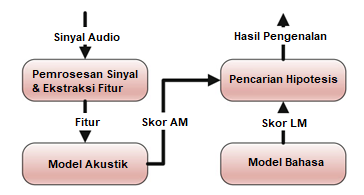
\includegraphics[width=0.8\textwidth]{resources/images/arsitektur-umum-asr.png}
    \caption{Arsitektur umum dari sistem ASR \parencite{Yu2014}}
\end{figure}


\subsection{Pemrosesan Sinyal dan Ekstraksi Fitur}

Komponen pemrosesan sinyal dan ekstraksi fitur mengambil masukan berupa sinyal audio mentah dan diproses agar \textit{noise}-nya dihilangkan, mengubah sinyal dari domain waktu ke domain frekuensi, dan mengekstraksi fitur-fitur yang paling penting dari sinyal tersebut sehingga cocok dengan komponen model akustik.

\subsection{Model Akustik}

Komponen model akustik tersebut mengintegrasikan pengetahuan mengenai akustik dan fonetik, dan dengan menggunakan fitur yang diekstraksi di komponen sebelumnya lalu menghasilkan skor AM untuk fitur tersebut.
\bigskip

Riset \textcite{Han2018} menunjukkan bahwa model akustik dengan \textit{word error rate} (WER) terbaik untuk korpus bahasa Inggris yaitu sebesar 5.0\% pada dataset Switchboard dan 9.1\% pada dataset CallHome, didapatkan dengan menggunakan dense TDNN-LSTM. Fitur yang digunakan adalah MFCC dengan dimensi sebesar 39, sama seperti yang dilakukan oleh \textcite{Xiong2017} akan tetapi model akustik yang digunakan adalah CNN-BLSTM.
\bigskip

Selain itu, terdapat riset lain yang menggunakan pendekatan \textit{sequence-to-sequence}, seperti \textcite{Chan2015} yang menggunakan \textit{Bidirectional} LSTM (BLSTM) dengan struktur piramid untuk mendapatkan representasi tingkat tinggi dari sinyal audio. Struktur piramid digunakan untuk mengurangi \textit{time-step} yang dibutuhkan untuk mendapatkan representasi dari keseluruhan sinyal audio, yang bisa mencapai ribuan pada sistem ASR. BLSTM struktur piramid tersebut pada pendekatan \textit{sequence-to-sequence} disebut sebagai \textit{encoder}, menghasilkan context vectors yang kemudian digunakan pada \textit{decoder} untuk menghasilkan rangkaian kata-kata sebagai hasil pengenalan. Model ini berhasil mencapai WER 14.1\% tanpa menggunakan kamus dan model bahasa, dan berhasil mencapai WER 10.3\% jika menggunakan model bahasa. Riset lain yang menggunakan pendekatan \textit{sequence-to-sequence} pada data bahasa Inggris adalah riset \textcite{Chung2017}, yang sama seperti riset sebelumnya hanya saja pada \textit{decoder}-nya tidak menerima masukan berupa sinyal audio mentah, tetapi sudah diekstraksi fitur terlebih dahulu menjadi fitur MFCC berdimensi 13 dengan urutan waktu terbalik. Model ini berhasil mencapai WER 17.7\% pada dataset LRS.
\bigskip

Riset mengenai ASR pada bahasa Indonesia salah satunya adalah oleh \textcite{Yuwan2018}, yang menggunakan model DNN-HMM dan dibandingkan dengan model tolak ukur GMM-HMM. Pengujian model dilakukan pada skema tertutup dan terbuka, dan berhasil mencapai penurunan WER dari ASR berbasis GMM-HMM ke ASR berbasis DNN-HMM sebesar 2,53\% pada skema tertutup dan 3,89\% pada skema terbuka.


\subsection{Model Bahasa}

Komponen model bahasa mengestimasi probabilitas dari rangkaian kata-kata hipotesis dengan cara mempelajari korelasi antar kata-kata tersebut berdasarkan korpus data latih. Estimasi probabilitas tersebut disebut sebagai skor LM.


\subsection{Pencarian Hipotesis}

Dengan menggunakan skor AM dan LM yang didapatkan dari vektor fitur dan kata-kata kandidat yang mungkin, komponen pencarian hipotesis akan menghasilkan keluaran berupa rangkaian kata-kata dengan skor AM dan LM tertinggi sebagai hasil pengenalan. 


\section{Pemodelan \textit{Sequence}}

Pemodelan \textit{sequence} dengan \textit{deep learning} berkembang dengan pesat, terutama menggunakan \textit{recurrent neural network} (RNN), yang telah menunjukkan hasil yang baik pada banyak permasalahan pembelajaran mesin, khususnya untuk permasalahan yang memiliki masukan dan/atau keluaran yang memiliki panjang yang bervariasi. Riset \textcite{Sutskever2014} dan \textcite{Bahdanau2015} menunjukkan bahwa RNN dapat melakukan pemodelan \textit{sequence} dengan baik sama seperti sistem-sistem yang sudah ada untuk permasalahan sulit seperti mesin translasi.
\bigskip

RNN merupakan perluasan dari jaringan saraf tiruan \textit{feedforward} konvensional yang dapat menangani masukan dengan panjang bervariasi. RNN menanganinya dengan menggunakan \textit{recurrent hidden} state yang pengaktifannya bergantung pada \textit{hidden state} pada waktu yang sebelumnya. Secara formal, RNN memperbarui \textit{recurrent hidden state} ht-nya sebagai berikut \parencite{Chung2014}:

\[ h_{t} =
  \begin{cases}
    0                           & \quad t=0 \\
    \varphi(h_{t-1} - x_{t})    & \quad otherwise
  \end{cases}
\]

yang pada hal ini \(x\) adalah rangkaian \(x=(x_{1},x_{2}\dots,x_{T})\) dan \(\varphi\) merupakan fungsi non-linier seperti fungsi \textit{logistic sigmoid}. RNN juga bisa memiliki keluaran \(y=(y_{1},y_{2}\dots,y_{T})\) yang juga memiliki panjang yang bervariasi.
\bigskip

Bobot atau parameter yang terdapat pada RNN secara tradisional diperbarui sebagai berikut \parencite{Chung2014}:
\[
    h_{t} = g(Wx_{t}+Uh_{t-1})
\]
yang dalam hal ini \(g\) merupakan fungsi seperti \textit{logistic sigmoid} atau \textit{hyperbolic tangent}.
\bigskip

Akan tetapi, pelatihan RNN sulit dilakukan untuk menangkap dependensi yang jaraknya jauh karena nilai gradien pada RNN cenderung menghilang atau meningkat drastis. Hal ini membuat optimasi berbasis gradien menjadi sulit untuk dilakukan. Pendekatan yang bisa dilakukan untuk menangani masalah ini bisa dengan melakukan optimasi yang lain yang tidak berbasis gradien, seperti menggunakan \textit{stocahstic gradient desecent}. Pendekatan lainnya yang bisa dilakukan adalah menggunakan arsitektur RNN yang lain yang menggunakan fungsi aktivasi yang lebih mutakhir, seperti \textit{long short-term memory} (LSTM) \parencite{Hochreiter1997} dan \textit{gated recurrent unit} (GRU) \parencite{Cho2014a}.
\bigskip

Pemodelan \textit{sequence} yang paling banyak digunakan pada riset-riset terakhir ini adalah menggunakan model \textit{sequence-to-sequence} yang memetakan sebuah rangkaian masukan dengan panjang \(n\) menjadi rangkaian keluaran dengan panjang \(m\), dipopulerkan dalam penggunaanya untuk permasalahan terjemahan mesin.
\bigskip

Terdapat dua pendekatan umum untuk model \textit{sequence-to-sequence}, yaitu model \textit{encoder-decoder} berbasis rekurens dan model \textit{encoder-decoder} berbasis \textit{attention}.


\subsection{Model \textit{Encoder-Decoder} berbasis rekurens}

Model dasar \textit{sequence-to-sequence} diperkenalkan oleh \textcite{Cho2014b}, yang terdiri dari dua buah \textit{recurrent neural network} (RNN), yaitu \textit{encoder} yang bertugas untuk merepresentasikan rangkaian masukan menjadi sebuah \textit{fixed-length vector}, dan \textit{decoder} yang bertugas untuk menghasilkan rangkaian keluaran berdasarkan vektor yang didapatkan dari encoder tadi.

\begin{figure}[h]
    \centering
    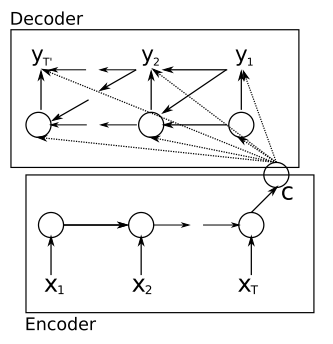
\includegraphics[width=0.8\textwidth]{resources/images/arsitektur-encoder-decoder.png}
    \caption{Ilustrasi dari arsitektur \textit{encoder-decoder} \parencite{Cho2014b}}
\end{figure}

Selain itu ada riset dari \textcite{Sutskever2014} yang sama menggunakan arsitektur \textit{encoder-decoder} akan tetapi berbeda dengan arsitektur sebelumnya yang hanya mengintegrasikan jaringan saraf tiruannya ke dalam sistem \textit{statistical machine translation} (SMT), model ini merupakan model yang sepenuhnya menggunakan RNN dan proses pelatihannya dilakukan secara \textit{end-to-end}. Hanya saja model \textit{encoder-decoder} ini harus dapat memampatkan informasi dari satu kalimat utuh menjadi sebuah \textit{fixed-length vector}. Hal ini bisa jadi menyulitkan RNN untuk merepresentasikan kalimat yang panjang, terutama jika panjangnya lebih panjang dari yang terdapat pada data latih di corpus. \textcite{Cho2014a} menunjukkan bahwa memang performa dari model \textit{encoder-decoder}-nya semakin memburuk seiring dengan semakin meningkatnya panjang dari kalimat masukan.
\bigskip

Untuk menangani masalah tersebut, \textcite{Bahdanau2015} mengaplikasikan mekanisme \textit{attention} pada \textit{decoder}. Dengan mekanisme \textit{attention} ini \textit{decoder} dapat menentukan bagian mana dari kalimat masukan yang harus mendapatkan perhatian lebih untuk selanjutnya menjadi masukan pada fungsi aktivasi pada \textit{decoder} untuk menentukan keluaran apa yang akan dihasilkan. Dengan membiarkan \textit{decoder} menentukan masukan mana yang penting untuk menghasilkan keluaran selanjutnya, \textit{decoder} menjadi tidak perlu untuk merepresentasikan semua informasi yang ada dalam sebuah kalimat ke dalam sebuah vektor. Dengan ini informasi pada sebuah kalimat bisa direpresentasikan secara tersebar ke seluruh rangkaian kata-kata pada kalimat, yang selanjutnya bisa dipilih oleh \textit{decoder} dengan mekanisme \textit{attention}.

\begin{figure}[h]
    \centering
    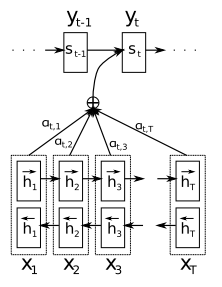
\includegraphics[width=0.8\textwidth]{resources/images/mekanisme-attention.png}
    \caption{Ilurstrasi mekanisme attention \parencite{Bahdanau2015}}
    \label{fig:attention}
\end{figure}

Seperti yang bisa dilihat pada gambar ~\ref{fig:attention}, tingkat kepentingan dari masukan dipilih oleh mekanisme \textit{attention} berdasarkan nilai dari bobot \(\alpha_{i,j}\) dari setiap masukan \(h_{j}\), yang dihitung dengan fungsi \textit{softmax} \parencite{Bahdanau2015}:

\[
    \alpha_{ij} = \frac{exp(e_{ij})}{\displaystyle\sum_{k=1}^{T_{}x} exp(e_{ik})}
\]

yang dalam hal ini,

\[
    e_{ij} = a(s_{i-1}, h_{j})
\]

yang merupakan model \textit{alignment} yang menilai kecocokan antara masukan pada sekitaran posisi \(j\) dan keluaran pada posisi \(i\). Parameter pada model \textit{alignment}  dilatih sebagai \textit{feedforward neural network} yang kemudian dilatih secara bersama-sama dengan komponen-komponen lain pada sistem yang diusulkan.


\subsection{Model \textit{Encoder-Decoder} berbasis \textit{attention}}

Mekanisme \textit{attention} sudah diaplikasikan pada berbagai permasalahan selain permasalahan mesin translasi dan menjadi bagian penting dalam pemodelan rangkaian dan model transduksi, sehingga memungkinkan model untuk memodelkan dependensi tanpa harus melihat jarak antara masukan dan keluaran. Akan tetapi, kebanyakan pengaplikasian mekanisme \textit{attention} ini hanya sebatas digunakan sebagai pelengkap untuk jaringan saraf rekuren. Oleh sebab itu \textcite{Vaswani2017} mengusulkan model yang disebut sebagai model transformer, sebuah arsitektur model yang menghindari penggunaan rekurens dan bergantung sepenuhnya pada mekanisme \textit{attention} untuk menggambarkan dependensi global antara masukan dan keluaran. Selain itu model transformer ini memungkinkan dilakukannya paralelisasi sehingga dapat mempercepat proses pelatihan model, dan juga berhasil mengungguli model \textit{encoder-decoder} berbasis rekurens.
\bigskip

Arsitektur dari model transformer secara keseluruhan mengikuti model \textit{encoder-decoder}, hanya saja komponen penyusunnya tidak menggunakan RNN tapi menggunakan \textit{stacked self-attention}, dan \textit{point-wise fully connected layer}. Selain itu untuk model transfromer juga tidak menggunakan RNN untuk meng-\textit{encode} rangkaian, tetapi menggunakan layer \textit{positional encodings} yang kemudian diikuti oleh fungsi \textit{attention}.
\bigskip

Fungsi \textit{attention} bisa dideskripsikan sebagai pemetaan \textit{query} dan sekumpulan pasangan \textit{key-value} menjadi sebuah keluaran, yang pada hal ini \textit{query}, pasangan \textit{key-value}, dan keluaran semuanya berbentuk vektor. Keluaran tersebut dihitung sebagai jumlah tertimbang. Jenis fungsi \textit{attention} yang digunakan pada riset ini disebut sebagai \textit{Scaled Dot-Product Attention}, yang kemudian fungsi \textit{attention} tersebut bisa dihitung secara paralel, yang kemudian disebut sebagai \textit{Multi-Head Attention}.

\begin{figure}[h]
    \centering
    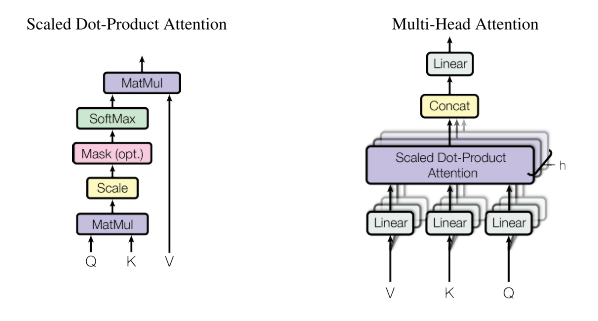
\includegraphics[width=0.8\textwidth]{resources/images/2-jenis-attention.png}
    \caption{Ilustrasi \textit{scaled dot-product attention} dan \textit{multi-head attention}. \parencite{Vaswani2017}}
    \label{fig:jenis-attention}
\end{figure}

\textit{Scaled dot-product attention}, mengambil input berupa beberapa \textit{query} (Q) dan \textit{key} (K) yang berdimensi \(d_{k}\), dan \textit{value} (V) yang berdimensi \(d_{v}\), dan dapat diformulasikan sebagai berikut:

\[
    Attention(Q,K,V) = \frac{QK^{T}}{\sqrt{d_{k}}}V    
\]

Pada dasarnya \textit{scaled dot-product attention} sama seperti \textit{dot-product attention}, perbedaannya terletak pada penambahan faktor penskala \(\frac{1}{d_{k}}\) pada perhitungannya. faktor penskala tersebut digunakan untuk menangani masalah ketika nilai  \(d_{k}\) terlalu besar sehingga hasil \textit{dot-product}nya tumbuh secara besar, sehingga hasil dari fungsi softmaxnya memiliki gradien yang sangat kecil dan selanjutnya menimbulkan masalah ketika melakukan propagasi balik.
\bigskip

\textit{Multi-head attention} merupakan pengembangan dari \textit{scaled dot-product attention}. Menurut \textcite{Vaswani2017}, daripada menghitung satu kali \textit{attention} dari \textit{query}, \textit{key}, dan \textit{value} yang sebanyak \(d_{model}\), akan lebih baik jika \textit{query}, \textit{key}, dan \textit{value}nya diproyeksikan secara linier terlebih dahulu sebanyak \(h\) kali, dengan proyeksi liner ke dimensi \(d_{q}\), \(d_{k}\), \(d_{v}\) dan  yang berbeda-beda dan dipelajari dari data. Masing-masing \textit{query}, \textit{key}, dan \textit{value} yang sudah diproyeksikan tersebut kemudian dihitung \textit{attention}nya secara paralel, dan menghasilkan output berdimensi \(d_{v}\) yang kemudian dikonkatenasi dan diproyeksikan lagi, yang merupakan hasil akhir dari perhitungan \textit{multi-head attention}. \textit{Multi-head attention} dapat diformulasikan sebagai berikut:

\begin{equation*}
    \begin{split}
        MultiHead(Q,K,V) = Concat(head_{1},\dots,head_{h})W^{O} \\
        head_{i} = Attention(QW^{Q}_{i},KW^{K}_{i},VW^{V}_{i})
    \end{split}
\end{equation*}

yang dalam hal ini \(QW^{Q}_{i}\), \(KW^{K}_{i}\), dan \(VW^{V}_{i}\) merupakan matrix parameter untuk proyeksi, yang dipelajari dari data.
\bigskip

Jenis \textit{attention} ini memungkinkan model untuk mempelajari informasi mana yang paling perlu diperhatikan dari berbagai representasi pada ruang pencarian dengan posisi yang berbeda-beda.

Selain menggunakan fungsi \textit{attention}, setiap layer pada \textit{encoder} dan \textit{decoder} berisi \textit{fully connected feedforward network}, yang terdiri dari dua transformasi linier dengan fungsi aktivasi ReLU diantaranya. Di layer masukan terdapat layer \textit{embedding} dan di layer keluaran digunakan layer softmax. Karena modelnya tidak mempunyai komponen rekurens atau konvolusi, supaya modelnya mampu mempelajari urutan dari rangkaiannya, maka modelnya harus dimasukkan informasi tambahan mengenai posisi relatif dan posisi absolut dari token di dalam sebuah kalimat. Untuk itu digunakan \textit{positional embedding} setelah melalui \textit{embedding} di layer masukan tadi.

\begin{figure}[h]
    \centering
    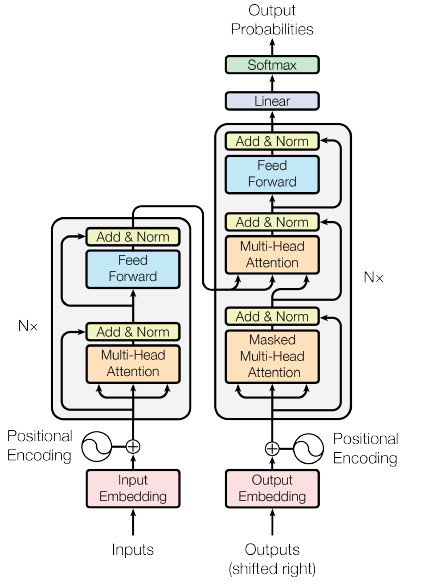
\includegraphics[width=0.8\textwidth]{resources/images/arsitektur-transformer.png}
    \caption{Arsitektur model Transformer \parencite{Vaswani2017}}
    \label{fig:transformer}
\end{figure}


\section{Pemodelan Gambar dan Video}

Riset yang paling banyak mengenai pemodelan gambar dan video adalah mengenai pembangkitan keterangan otomatis (\textit{automatic caption generation}). Pembangkitan keterangan otomatis merupakan permasalahan mendasar pada kecerdasan buatan yang menggabungkan \textit{computer vision} dan pemrosesan bahasa alami. Riset mengenai pembangkitan keterangan otomatis akhir-akhir ini bisa dikategorisasikan menjadi dua, yaitu pembangkitan keterangan otomatis dari citra dan pembangkitan keterangan otomatis dari video. Jika proses pembangkitan dilakukan dari citra maka informasi penting yang harus diperhatikan hanya informasi posisi saja sedangkan jika dilakukan dari video maka selain itu harus juga diperhatikan informasi temporal antar frame videonya. Permasalahan utamanya adalah sebuah deskripsi dihasilkan harus bisa menangkap semua objek yang terdapat di dalam citra tersebut, dan juga harus bisa mengekspresikan keterkaitan antara objek dan juga atribut-atribut apa saja yang menjelaskan objek tersebut dan aktivitas apa yang melibatkan objek tersebut. Terlebih lagi, deskripsi tersebut harus dideskripsikan dengan menggunakan bahasa yang sealami mungkin.


\subsection{Pembangkitan Keterangan Otomatis dari Citra}

Riset \textcite{Vinyals2014} mengemukakan sebuah model yang diinspirasi oleh kemajuan-kemajuan terbaru pada permasalahan mesin translasi yang menggunakan model \textit{encoder-decoder} berbasis RNN. Perbedaannya pada riset ini adalah sebagai ganti dari RNN, modelnya menggunakan \textit{convolutional neural network} (CNN) sebagai encoder. Dalam beberapa tahun terakhir penggunaan CNN telah menunjukkan hasil yang baik dalam merepresentasikan sebuah citra menjadi sebuah \textit{fixed-length vector}, sehingga selanjutnya bisa digunakan sebagai masukan dari \textit{decoder} RNN untuk menghasilkan keluaran berupa kalimat deskripsi.
/bigskip

CNN merupakan bagian dari \textit{deep feedforward artificial neural networks} yang pada umumnya digunakan untuk menganalisis citra. CNN merupakan variasi dari \textit{multilayer perceptron} dan didesain supaya memerlukan praproses seminimal mungkin. CNN terdiri dari banyak lapisan tersembunyi yang melakukan konvolusi dan \textit{pooling} terhadap masukan yang pada umumnya berbentuk citra. Lapisan-lapisan konvolusi dan \textit{pooling} ini memiliki nilai-nilai parameter yang dipelajari dari data sehingga Lapisan-lapisan tersebut secara otomatis menyesuaikan untuk bisa mengekstraksi informasi yang paling penting. Pada CNN, lapisan tersembunyinya biasanya terdiri atas lapisan konvolusi, lapisan \textit{pooling}, \textit{fully connected layers} dan lapisan normalisasi. 
\bigskip

Lapisan konvolusi menggunakan operasi konvolusi kepada masukan, dan meneruskan hasilnya ke lapisan selanjutnya. Setiap lapisan konvolusi memproses data hanya pada \textit{receptive field}nya. \textit{Receptive field} adalah sebagian area dari keseluruhan data yang akan diproses. Area tersebut biasanya berbentuk persegi. \textit{Receptive field} digunakan untuk mengurangi jumlah parameter jika dibandingkan dengan menggunakan \textit{fully connected layer}, karena ukuran dari sebuah citra yang biasanya berukuran besar, dan setiap pixelnya merupakan input yang relevan.
\bigskip

Lapisan \textit{pooling} pada CNN bertugas untuk menggabungkan kluster neuron dari lapisan keluaran sebelumnya menjadi satu neuron pada layer selanjutnya. Misalnya, pada lapisan m\textit{max-pooling} diambil nilai maksimum dari setiap kluster di lapisan sebelumnya. Contoh lainnya adalah lapisan \textit{average-pooling} yang mengambil nilai rata-rata dari setiap kluster di lapisan sebelumnya.

\begin{figure}[h]
    \centering
    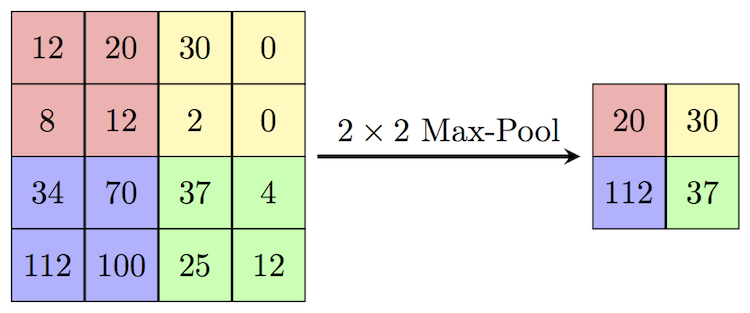
\includegraphics[width=0.8\textwidth]{resources/images/max-pooling.png}
    \caption{Ilustrasi lapisan \textit{max-pooling}}
    \label{fig:max-pooling}
\end{figure}

\textit{Fully connected layer} cara kerjanya sama seperti \textit{multilayer perceptron}, menghubungkan setiap neuron pada lapisan sebelumnya ke setiap neuron yang ada pada lapisan setelah lapisan tersebut.
\bigskip

Diinspirasi lebih lanjut dari permasalahan mesin translasi yang menggunakan mekanisme \textit{attention}, riset \textcite{Xu2015} mengembangkan lebih lanjut riset \textcite{Vinyals2014} dengan memberikan mekanisme \textit{attention} pada saat \textit{decoder} melakukan pembangkitan deskripsi dari citra.

\begin{figure}[h]
    \centering
    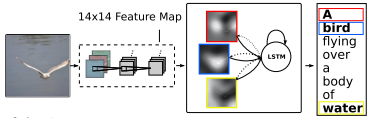
\includegraphics[width=0.8\textwidth]{resources/images/image-captioning-encoder-decoder.png}
    \caption{Ilustrasi model \textit{encoder-decoder} dengan menggunakan \textit{attention} pada \textit{image captioning} \parencite{Xu2015}.}
    \label{fig:image-captioning-encoder-decoder}
\end{figure}


\subsection{Pembangkitan Keterangan Otomatis dari Video}

Riset lain yang juga terinspirasi dari perkembangan terkini dalam mesin translasi adalah riset mengenai pembangkitan keterangan otomatis dari video yang dilakukan oleh \textcite{Venugopalan2015}. Model yang dikemukakan menggunakan model \textit{seqence-to-sequence} dengan \textit{recurrent network} yang digunakan sebagai \textit{decoder} dan \textit{encoder}-nya adalah LSTM bertumpuk. Masukan dari LSTM bertumpuk tersebut berupa citra RGB dan informasi \textit{optical flow} yang kemudian keduanya direpresentasikan menjadi sebuah \textit{embedding} dengan menggunakan CNN yang parameternya dilatih bersama-sama dengan parameter yang terdapat pada LSTM bertumpuk.
\bigskip

\begin{figure}[h]
    \centering
    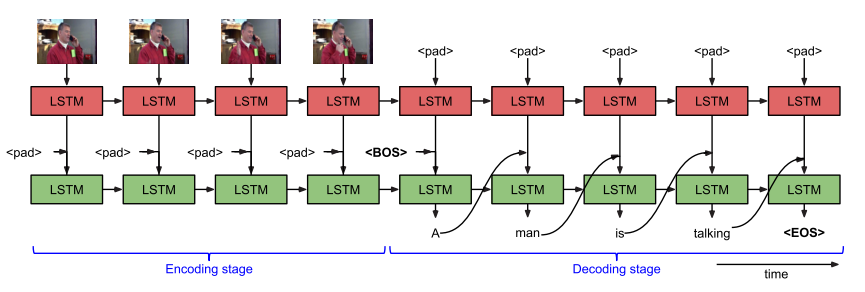
\includegraphics[width=0.8\textwidth]{resources/images/video-to-text.png}
    \caption{Ilustrasi model \textit{video-to-text} \parencite{Chung2017}.}
    \label{fig:video-to-text}
\end{figure}

Selain itu ada riset lain yang tidak menggunakan \textit{recurrent network} tetapi menggunakan CNN yang telah dimodifikasi untuk dapat memanfaatkan informasi spasial dan temporal pada video, sehingga diberi nama \textit{spatio-temporal convolutional neural network} (STCNN) \parencite{Karpathy2014}. Cara kerjanya sama seperti CNN hanya saja keterhubungan jaringannya diperluas pada dimensi waktunya sehingga model dapat mempelajari fitur spatio-temporal. Perluasannya tersebut dibagi menjadi tiga, yaitu \textit{early fusion}, \textit{late fusion}, dan \textit{slow fusion}.

\begin{figure}[h]
    \centering
    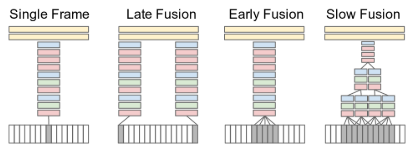
\includegraphics[width=0.8\textwidth]{resources/images/stcnn.png}
    \caption{Ilustrasi STCNN \parencite{Karpathy2014}.}
    \label{fig:stcnn}
\end{figure}

Pada \textit{early fusion}, modelnya menggabungkan informasi temporal di seluruh frame dengan \textit{window} yang telah ditentukan, langsung pada tingkat pixel. Sedangkan pada \textit{late fusion}, dari \textit{window} yang telah ditentukan diambil dua buah frame, frame awal dan frame akhir, lalu masing-masing frame melalui berbagai lapisan konvolusi, lalu menggabungkan kedua representasi yang didapatkan dengan menggunakan \textit{fully connected layer}. Untuk \textit{slow fusion}, merupakan model yang menggabungkan dua pendekatan tadi (\textit{early fusion} dan \textit{late fusion}) dengan cara menggabungkan informasi temporal dari semua frame pada \textit{window} secara perlahan-lahan dan hirarkis.


\section{\textit{Visual Speech Recognition}}

Riset \textcite{Chung2017} melakukan task pembangkitan keterangan otomatis dari video yang cakupannya lebih kecil, yaitu melakukan pengenalan gerak bibir untuk \textit{visual speech recognition}. Model yang digunakan dapat dibagi menjadi tiga modul, yaitu modul \textit{Watch}, modul \textit{Listen}, modul \textit{Attend}, dan modul \textit{Spell}, dan bisa diformalisasikan sebagai berikut \parencite{Chung2017}:

\begin{equation*}
    \begin{split}
        s^{v}, o^{v} &= Watch(x^{v}) \\
        s^{a}, o^{a} &= Listen(x^{a}) \\
        P(y|x^{v}, x^{a}) &= Spell(s^{v}, s^{a}, o^{v}, o^{a})
    \end{split}
\end{equation*}

Modul \textit{Watch}, merupakan \textit{encoder} citra yang terdiri atas modul konvolusi yang menghasilkan fitur citra \(f^{v}_{i}\) untuk setiap masukan di \textit{time-step} \(x^{v}_{i}\), ditambah dengan sebuah modul rekuren yang menghasilkan fixed-length vector \(s^{v}\) dan sekumpulan vektor output \(o^{v}\).
\bigskip

Modul \textit{Listen}, merupakan \textit{encoder} yang berisi sama seperti modul \textit{Watch} tetapi tanpa memiliki modul konvolusi. Modul rekurennya menerima masukan berupa hasil ekstraksi fitur menggunakan MFCC berdimensi 13, lalu dari modul rekuren tersebut dihasilkan vektor berukuran tetap \(s^{a}\) dan sekumpulan vektor keluaran \(o^{a}\).
\bigskip

Modul \textit{Spell}, berbasis pada transduser LSTM dan menghasilkan keluaran berupa rangkaian token pada level karakter. Modul ini bisa diformulasikan sebagai berikut \parencite{Chung2017}.

\begin{equation*}
    \begin{split}
        h^{d}_{k}, h^{d}_{k} &= LSTM(h^{d}_{k-1}, y_{k-1}, c^{v}_{k-1}, c^{a}_{k-1}) \\
        c^{v}_{k} &= o^{v} \cdot Attention^{v}(h^{d}_{k}, o^{v}) \\
        c^{a}_{k} &= o^{a} \cdot Attention^{a}(h^{d}_{k}, o^{a}) \\
        P(y_{i} | x^{v}, x^{a}, y_{<i}) &= softmax(MLP(o^{d}_{k}, c^{v}_{k}, c^{a}_{k}))
    \end{split}
\end{equation*}

\begin{figure}[h]
    \centering
    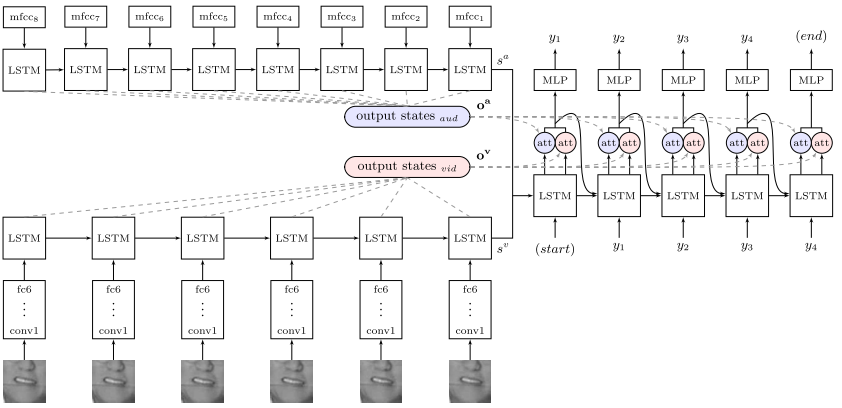
\includegraphics[width=0.8\textwidth]{resources/images/wlas.png}
    \caption{Arsitektur model \textit{Watch}, \textit{Listen}, \textit{Attend}, dan \textit{Spell} \parencite{Chung2017}.}
    \label{fig:wlas}
\end{figure}
    % \chapter{Analisis Masalah dan Perancangan Solusi}

\section{Analisis \textit{Speech Recognition}}

Ada beberapa permasalahan yang ditemukan pada permasalahan pengenalan ucapan, dan salah satunya dan yang menjadi fokus pada riset ini adalah kesulitan sistem pengenal ucapan dalam mengenali suara pada lingkungan yang bising. Beberapa riset-riset terkait mengenai permasalahan tersebut mencoba untuk menyelesaikannya dengan menambahkan informasi visual pada proses pengenalan suaranya, seperti pada riset \textcite{Chung2017}, \textcite{Chung2016}, dan \textcite{Assael2016}.
\bigskip

Untuk riset-riset yang menggunakan bahasa Indonesia sejauh ini sudah banyak yang menggunakan pendekatan \textit{deep learning} akan tetapi belum ada riset yang menggabungkan fitur akustik dan fitur visual, baik yang menggunakan fitur \textit{handcrafted} dan model akustik berbasis statistik maupun \textit{deep learning}.


\section{Analisis \textit{Lip Reading}}

Riset-riset terkait \textit{lip reading} bahasa Indonesia masih terbilang sedikit jika dibandingkan dengan riset-riset \textit{lip reading} dengan bahasa lain, terutama bahasa Inggris. Riset mengenai \textit{lip reading} yang menggunakan dataset bahasa Indonesia kebanyakan masih belum menggunakan \textit{deep learning}, seperti pada riset \textcite{Achmad2015} yang menggunakan HMM menunjukkan bahwa hasil pengenalan masih belum tergeneralisasi dengan baik karena hasilnya masih berpengaruh pada kondisi bibir pembicara, yang dalam hal ini pembicara wanita dengan bibir yang menggunakan lipstik memiliki koefisien korelasi yang tinggi sedangkan untuk yang bibir berwarna pucat dan bibir yang memiliki kumis di atasnya memiliki koefisien korelasi yang rendah.
\bigskip

Selain riset tersebut, pada saat penulisan, hanya ada satu paper mengenai \textit{lip reading} dalam bahasa Indonesia yang menggunakan pendekatan \textit{deep learning}, yaitu oleh \textcite{Maulana2018}, yang menggunakan \textit{spatiotemporal} CNN untuk menangkap struktur \textit{spatiotemporal} dari video, dan menggunakan \textit{bidirectional} Gated Recurrent Unit (GRU) untuk memodelkan keseluruhan rangkaian frame video dari dua arah, baik dengan urutan frame normal maupun dengan urutan terbalik.


\section{Analisis Model \textit{sequence-to-sequence}}

Salah satu permasalahan yang ditemui dalam penggunaan model \textit{sequence-to-sequence} untuk mentransduksi sebuah rangkaian menjadi rangkaian lain adalah kebanyakan model ini menggunakan RNN atau variannya sehingga prosesnya tidak bisa diparalelisasi karena sifatnya yang rekurens. Oleh sebab itu, proses pelatihan model membutuhkan waktu yang lama hingga model akhirnya konvergen. Pada riset \textcite{Vaswani2017} di usulkan model yang disebut sebagai model transformer, sebuah arsitektur model yang menghindari penggunaan rekurens dan bergantung sepenuhnya pada mekanisme \textit{attention} untuk menggambarkan dependensi global antara masukan dan keluaran. Selain itu model transformer ini memungkinkan dilakukannya paralelisasi sehingga dapat mempercepat proses pelatihan model, dan juga berhasil mengungguli model \textit{encoder-decoder} berbasis RNN dalam mentransduksi rangkaian.

\section{Usulan Solusi}

Berikut adalah rancangan arsitektur penyelesaian permasalahan pengenalan suara dengan menggunakan fitur akustik dan visual pada bahasa Indonesia.

\begin{figure}[h]
    \centering
    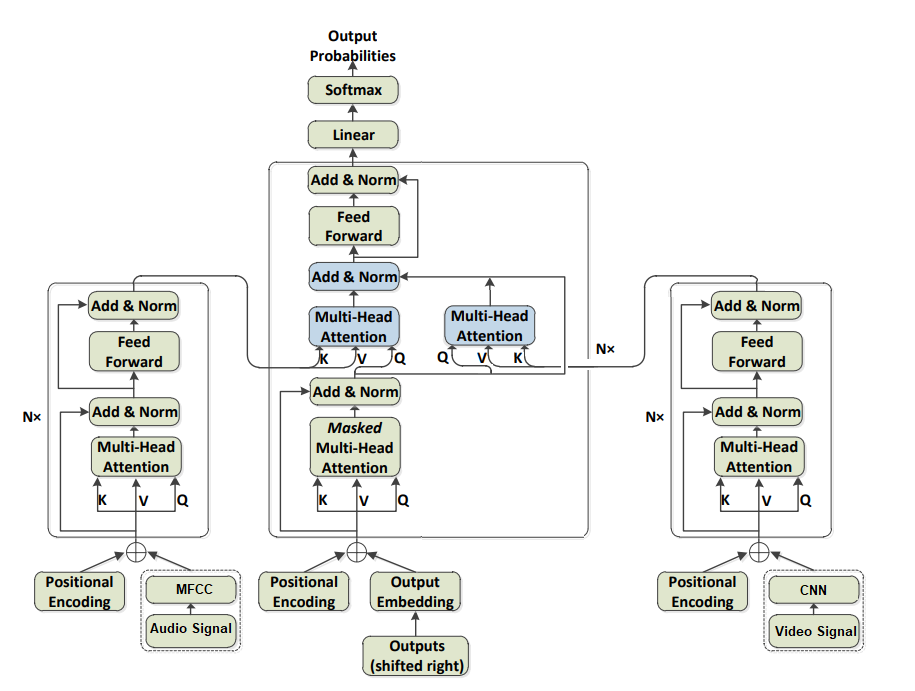
\includegraphics[width=0.8\textwidth]{resources/images/usulan-arsitektur.png}
    \caption{Rancangan Arsitektur.}
    \label{fig:usulan-arsitektur}
\end{figure}

Rangkaian penyelesaiannya adalah sebagai berikut.
\begin{enumerate}
    \item Melakukan perancangan model akustik dengan menggunakan model transformer (Gambar \ref{fig:usulan-arsitektur}) dan melakukan pelatihan model menggunakan dataset dalam bahasa Indonesia. Masukan yang digunakan adalah \textit{raw speech} yang kemudian diekstraksi fiturnya dengan menggunakan MFCC.
    \item Melakukan perancangan model untuk bagian \textit{visual speech recognition} dengan menggunakan model transformer (Gambar \ref{fig:usulan-arsitektur}) dan melakukan pelatihan model menggunakan dataset dalam bahasa Indonesia. Masukan yang digunakan adalah frame video yang direpresentasikan menjadi \textit{fixed-length vector} dengan menggunakan CNN.
    \item Melakukan penggabungan kedua model ASR dan VSR, dan melakukan pelatihan secara bersama-sama.
\end{enumerate}

Metrik pengujian yang digunakan pada saat pengujian adalah \textit{word error rate} (WER). Pengujian dilakukan dengan membandingkan model ASR dengan model \textit{baseline}nya, lalu selanjutnya melakukan perbandingan model VSR dengan model \textit{baseline}nya, lalu terakhir adalah melakukan pengujian terhadap model gabungan ASR dan VSR dan dibandingkan dengan model ASR saja, model VSR saja, dan \textit{baseline} dari model gabungan ASR dan VSR.

\section{Analisis Masalah}
\blindtext

\section{Solusi Umum}
\blindtext

\section{Rancangan Solusi}
\blindtext
    \chapter{Eksperimen dan Evaluasi}

\section{Tujuan Pengujian}
\blindtext

\section{Skenario Pengujian}
\blindtext

\section{Hasil Pengujian}
\blindtext

\section{Pembahasan}
\blindtext
    % \chapter{Penutup}

\section{Kesimpulan}
\blindtext

\section{Saran}
\blindtext
    %----------------------------------------------------------------%

    % Daftar pustaka
    \setquotestyle{english}
    \printbibliography[heading=bibintoc,title=Daftar Pustaka]

    % Index
    % \appendix

    % \addcontentsline{toc}{part}{Lampiran}
    % \part*{Lampiran}
    % \chapter{Instrumen Pengujian}
    % \chapter{Rincian Kasus Uji}

\end{document}
